\scanpage{111}
Examinons \unsure{un peu} de près les parties \unsure{antifiques|antifinies} \inserted{(et loc. constructibles)} de $X$, quand on ne suppose pas $X$ q. cpt. .....

\figure{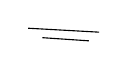
\begin{tikzpicture}[x=1cm,y=1cm]\draw(0,0)--(.9,-.05);\draw(.18,-.12)--(.77,-.16);\end{tikzpicture}}

\uline{\unsure{Pr.}} Soit $X$ un schéma affine. Alors $X^{\mathrm{cons}}$ est compact.

\uline{Corollaire 1} Soit $X$ un préschéma \deleted{\unsure{quelconque|noethérien}} \inserted{q. séparé}. Alors $X$ est $T_0$, admet une base formée d'ouverts rétrocompacts et compacts pour la topologie constructible. En partic., $X^{\mathrm{cons}}$ est loc. compact.

\uline{Corollaire \unsure{2|3}} Supposons \deleted{de plus} $X$ [quasi-compact et quasi-séparé] \deleted{Alors} quasi-noethérien. Alors

(i) $X^{\mathrm{cons}}$ est compact. (ii) les parties constructibles de $X$ sont les parties ouvertes et fermées de $X^{\mathrm{cons}}$.

(iii) les parties \deleted{\unsure{affines et}} \unsure{antifiques|antifinies} de $X$ sont les parties $E$ telles qu'il existe un morphisme q. cpt $f:X'\longrightarrow X$ d'image $E$.

On peut prendre \inserted{pour} \deleted{\unsure{$f$}} $X'\longrightarrow X$ un \uline{monomorphisme} q. cpt \unsure{...}

\deleted{[NB. \unsure{admet}} (iv) Si $E$ et $X-E$ ont cette propriété, ils sont constructibles ....

\margin{\figure{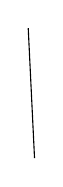
\begin{tikzpicture}[x=1cm,y=1cm]\draw(0,0)--(.08,-1.65);\end{tikzpicture}}}
\margin{110}
